\documentclass{acm_proc_article-sp}

\title{Screen-Camera Communications}
\subtitle{}
\author{
    Zhe-Yu Wu, Shao-Chuan Lee, Hsin-Wei Wang, Shao-Tung Chiu, Tsuen-Je Tsai \\
    \affaddr{B02902125, B01902010, B01902048, B01902085, B01902138} \\
    \email{\{B02902125, B01902010, B01902048, B01902085, B01902138\}@csie.ntu.edu.tw}
}

\begin{document}
\maketitle

\begin{abstract}
In this project, we will implement InFrame\cite{conf/hotnets/0002PZSZ14}, a screen-camera communication system. The system enables dual-mode full-frame communication for both humans and devices simultaneously, i.e., devices are able to receive encoded data while not interrupting normal screen display. Such a system is achieved by leveraging characteristics of human vision and high frame rate of modern display.
\end{abstract}

\section{Introduction}
In recent years, in order to take advantage of data-carrying capabilities of visual content, communication systems over visible channels have been developed. In applications such as Quick Response (QR) codes, end devices are able to retrieve information by capturing encoded images through cameras. However, due to limited display space, challenges are faced while attempting to allocate space for both visual contents for humans and encoded patterns for devices.

\begin{figure}[!h]
    \centering
    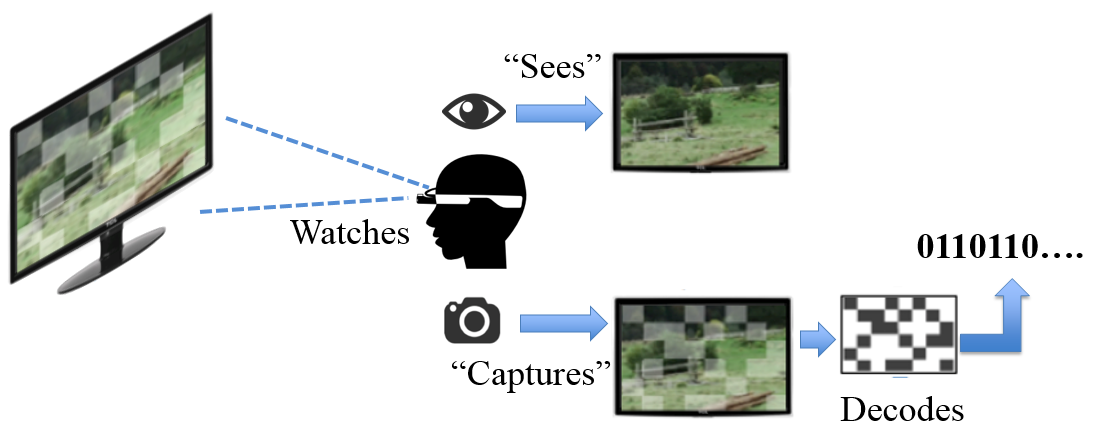
\includegraphics[width=\linewidth]{figures/concept}
    \caption{Concept of full-frame multiplexing}
    \label{fig:concept}
\end{figure}

To transmit both human-friendly and device-readable visual information simultaneously, a full-frame multiplexing scheme is proposed in InFrame. Figure \ref{fig:concept} illustrates the concept of the system, where the screen shows video frames multiplexed with data. Devices are able to capture and decode data from the video, while data transmission is unnoticable by humans.

Knowledge of human vision is essential for designing the system. Our visual perception possesses two features, the \textit{low-pass flicker fusion} and the \textit{phantom array effect}. For light flickering beyond a certain frequency (usually 40-50Hz), human eyes only perceive average luminance, acting like a low-pass filter. However, flicker at higher frequencies can be noticed if the object is fast-moving across view. The proposed multiplexing scheme in InFrame is aware of both properties, and tries to minimize human perception of multiplexed data.

\section{System Design}

\begin{figure}[!h]
    \centering
    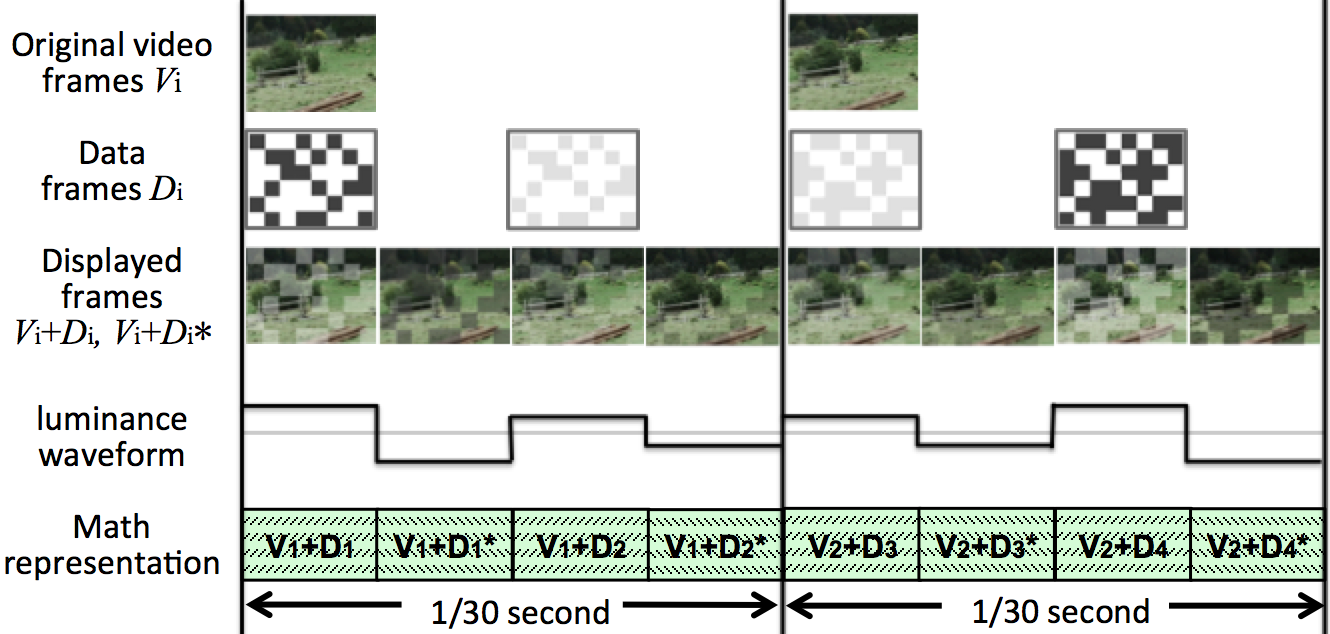
\includegraphics[width=\linewidth]{figures/design}
    \caption{Illustration of overall design in \textsc{InFrame}}
    \label{fig:design}
\end{figure}

In InFrame, an 120Hz display is used to deliver a 30FPS video clip. As shown in Figure \ref{fig:design}, 4 displayed frames are generated from 1 video frame and 2 data frames. Data frames consist of blocks, where a empty block denotes 0 and a ``chessboard pattern'' denotes 1. For each displayed frame composed of 1 video frame and 1 data frame, its \textit{complement} is displayed in the next frame such that the average luminance level of the two frames equals to that of the original video frame. To avoid phantom array effect, data frames fades out/in before/after switching to another.

During demultiplexing, the \textit{induced noise levels} of each block is calculated, which is the difference between smoothed block content and the original content. Since blocks carrying the chessboard pattern yields larger differences than empty ones, the bit information carried by a block can be identified.

\bibliographystyle{abbrv}
\bibliography{proposal}

\end{document}